\section{Edge triggered D Flip-Flop}

\subsection{Schematic}

Figure \ref{fig:dff_sch} shows the schematic and MOSFET parameters of the D Flip-Flop (DFF).

The transmission gate MOSFETs are sized as $2 \mu m$ for PMOS and $1 \mu m$ for NMOS, the same as the inverter.

\subsection{Simulation}

The DFF cell was simulated using the test bench schematic in laboratory notes. The inputs are set up to show all possible operations a DFF may do, including asynchronous resetting and latching both high and low level signals.

Figure \ref{fig:dff_trans} shows the transient simulation result. The waveform clearly shows the propagation delay between clock rising edge and a stable output is much less than $10 \mu s$, as required by $100 MHz$ operation.

\begin{figure}[!htb]
	\centering
	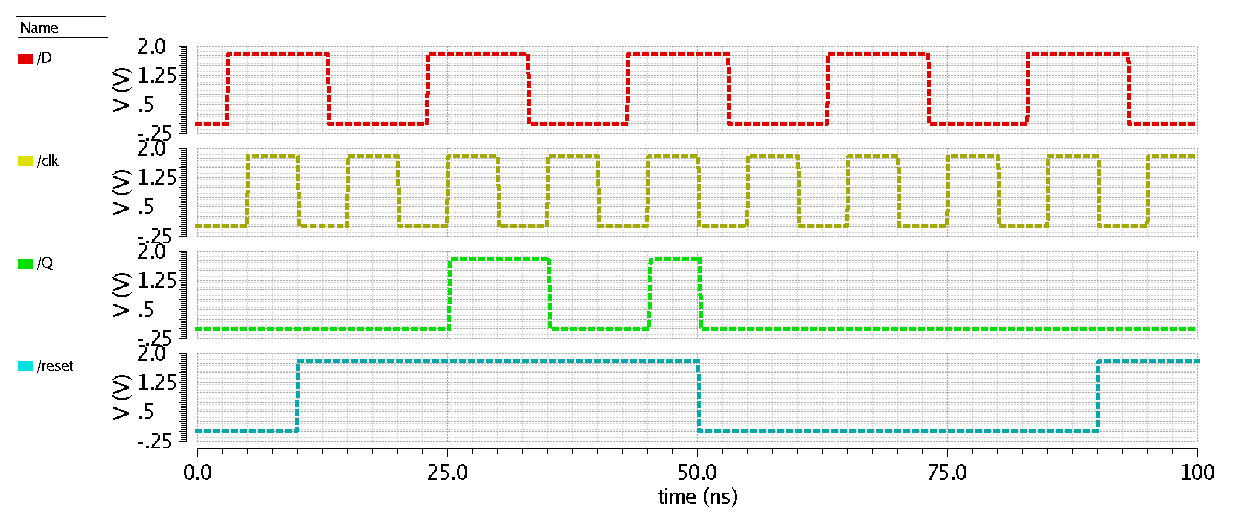
\includegraphics[width=\textwidth]{DFF_tb_trans}
	\caption{Transient simulation of the DFF design}
	\label{fig:dff_trans}
\end{figure}

\subsection{Layout}

Figure \ref{fig:dff_lay} shows the final layout design for the DFF cell. For reducing cell width, the standard cells are placed tightly next to each other, and the MOSFETs of the 4 transmission gates were combined as 2 groups. Several iterations, involving modifying the inverter and NAND layout design, reducing transmission gate PMOS transistors from 2 fingers to 1 finger, were made to achieve minimum cell width. The final cell size achieved was $26.64 \mu m \times 8 \mu m$.

While keeping the cell as compact as possible, the routings inside the cell were designed as thick as possible, especially for poly silicon layer routings. The sheet resistance for poly silicon is much higher than metal layer, therefore poly silicon routings should be kept as short and thick as possible. The gpdk180 reference manual states the sheet resistances for ploy and metal are 7.5 and 0.1 $\Omega / \text{square}$ respectively, it is very easy for a long thin ploy silicon trace to reach several kilo ohms of resistance. For this purpose, the VDD tap for the inverter was changed to the centre instead of 2 outer taps as in the example layout.

This layout design passed the DRC and LVS verification, as shown in Figure \ref{fig:dff_vfy}.

\begin{figure}[!htb]
	\centering
	\begin{subfigure}[b]{0.5\textwidth}
		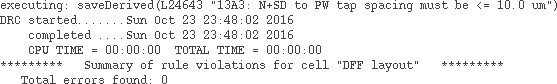
\includegraphics[width=\textwidth]{DFF_drc}
		\caption{DRC checking result, no errors}
		\label{fig:dff_drc}
	\end{subfigure}
	\begin{subfigure}[b]{0.4\textwidth}
		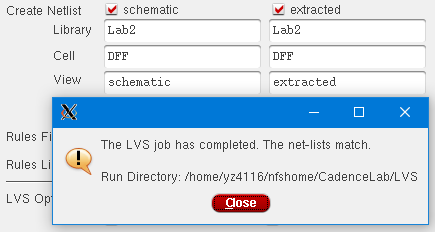
\includegraphics[width=\textwidth]{DFF_lvs}
		\caption{LVS checking result, the extracted net-list matches the schematic}
		\label{fig:dff_lvs}
	\end{subfigure}
	\caption{DFF cell layout verification}
	\label{fig:dff_vfy}
\end{figure}

\begin{sidewaysfigure}[!htb]
	\centering
	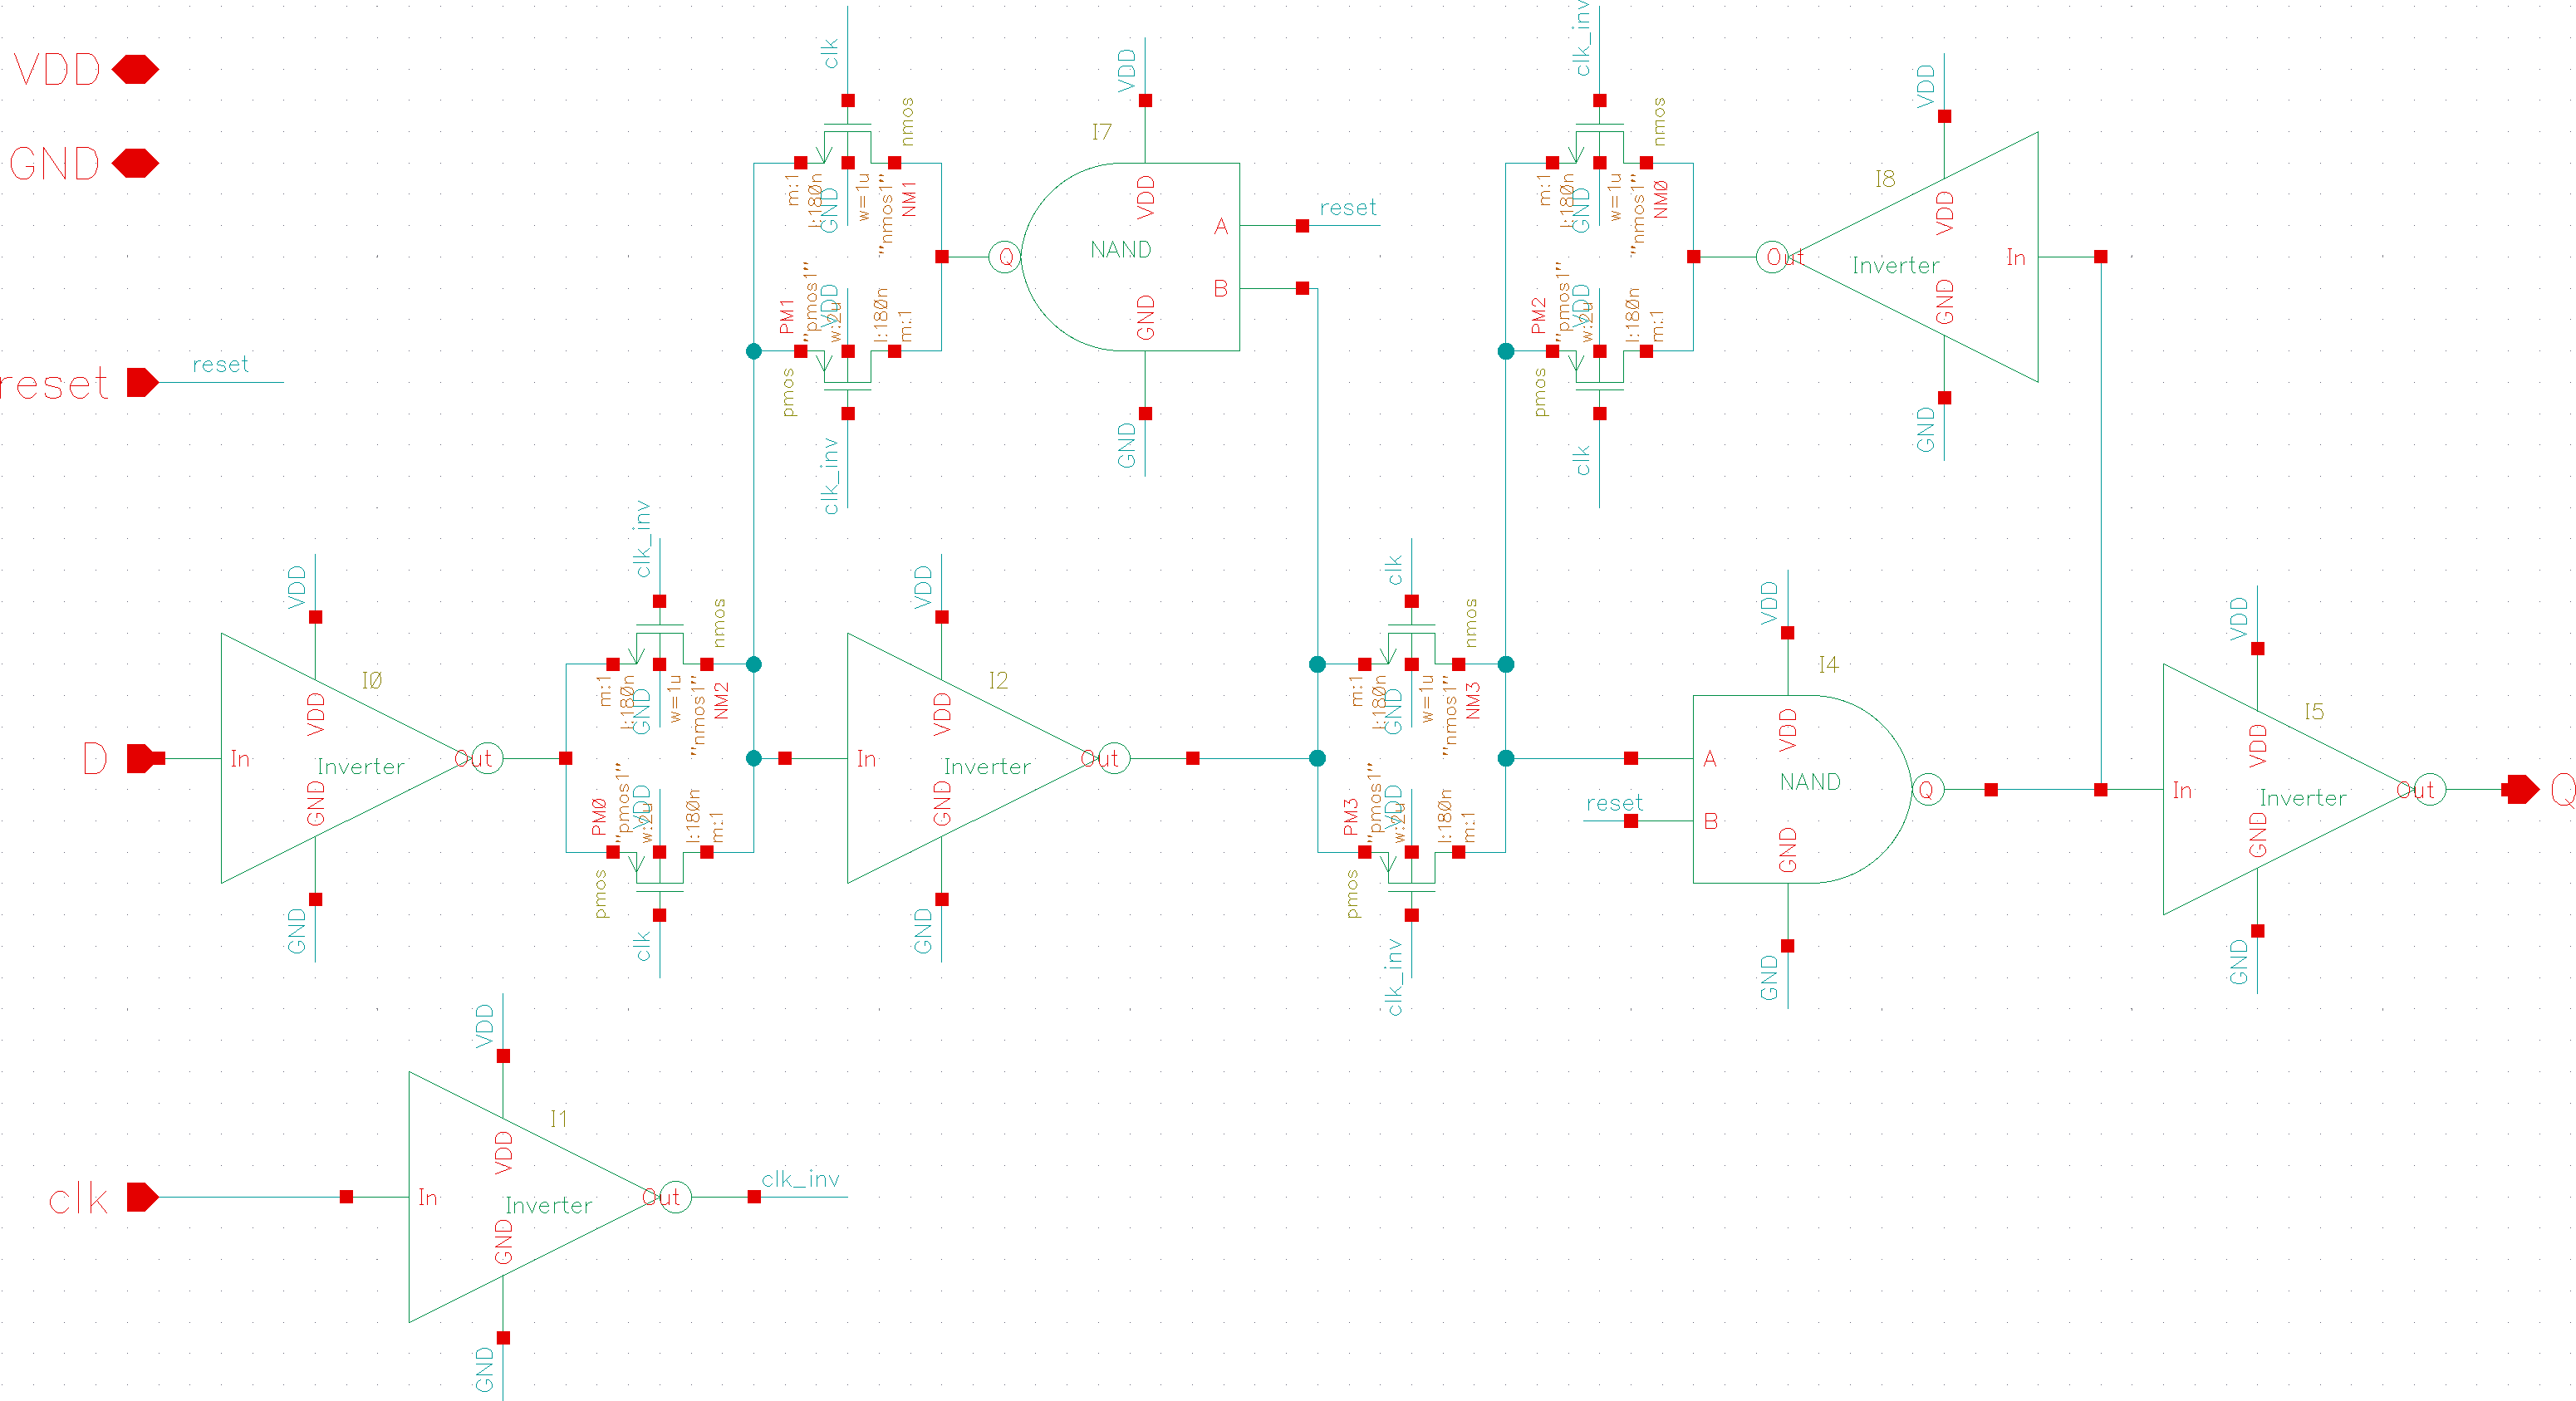
\includegraphics[width=\textwidth]{DFF_sch}
	\caption{Schematic of DFF including MOSFET parameters}
	\label{fig:dff_sch}
\end{sidewaysfigure}

\begin{sidewaysfigure}[!htb]
	\centering
	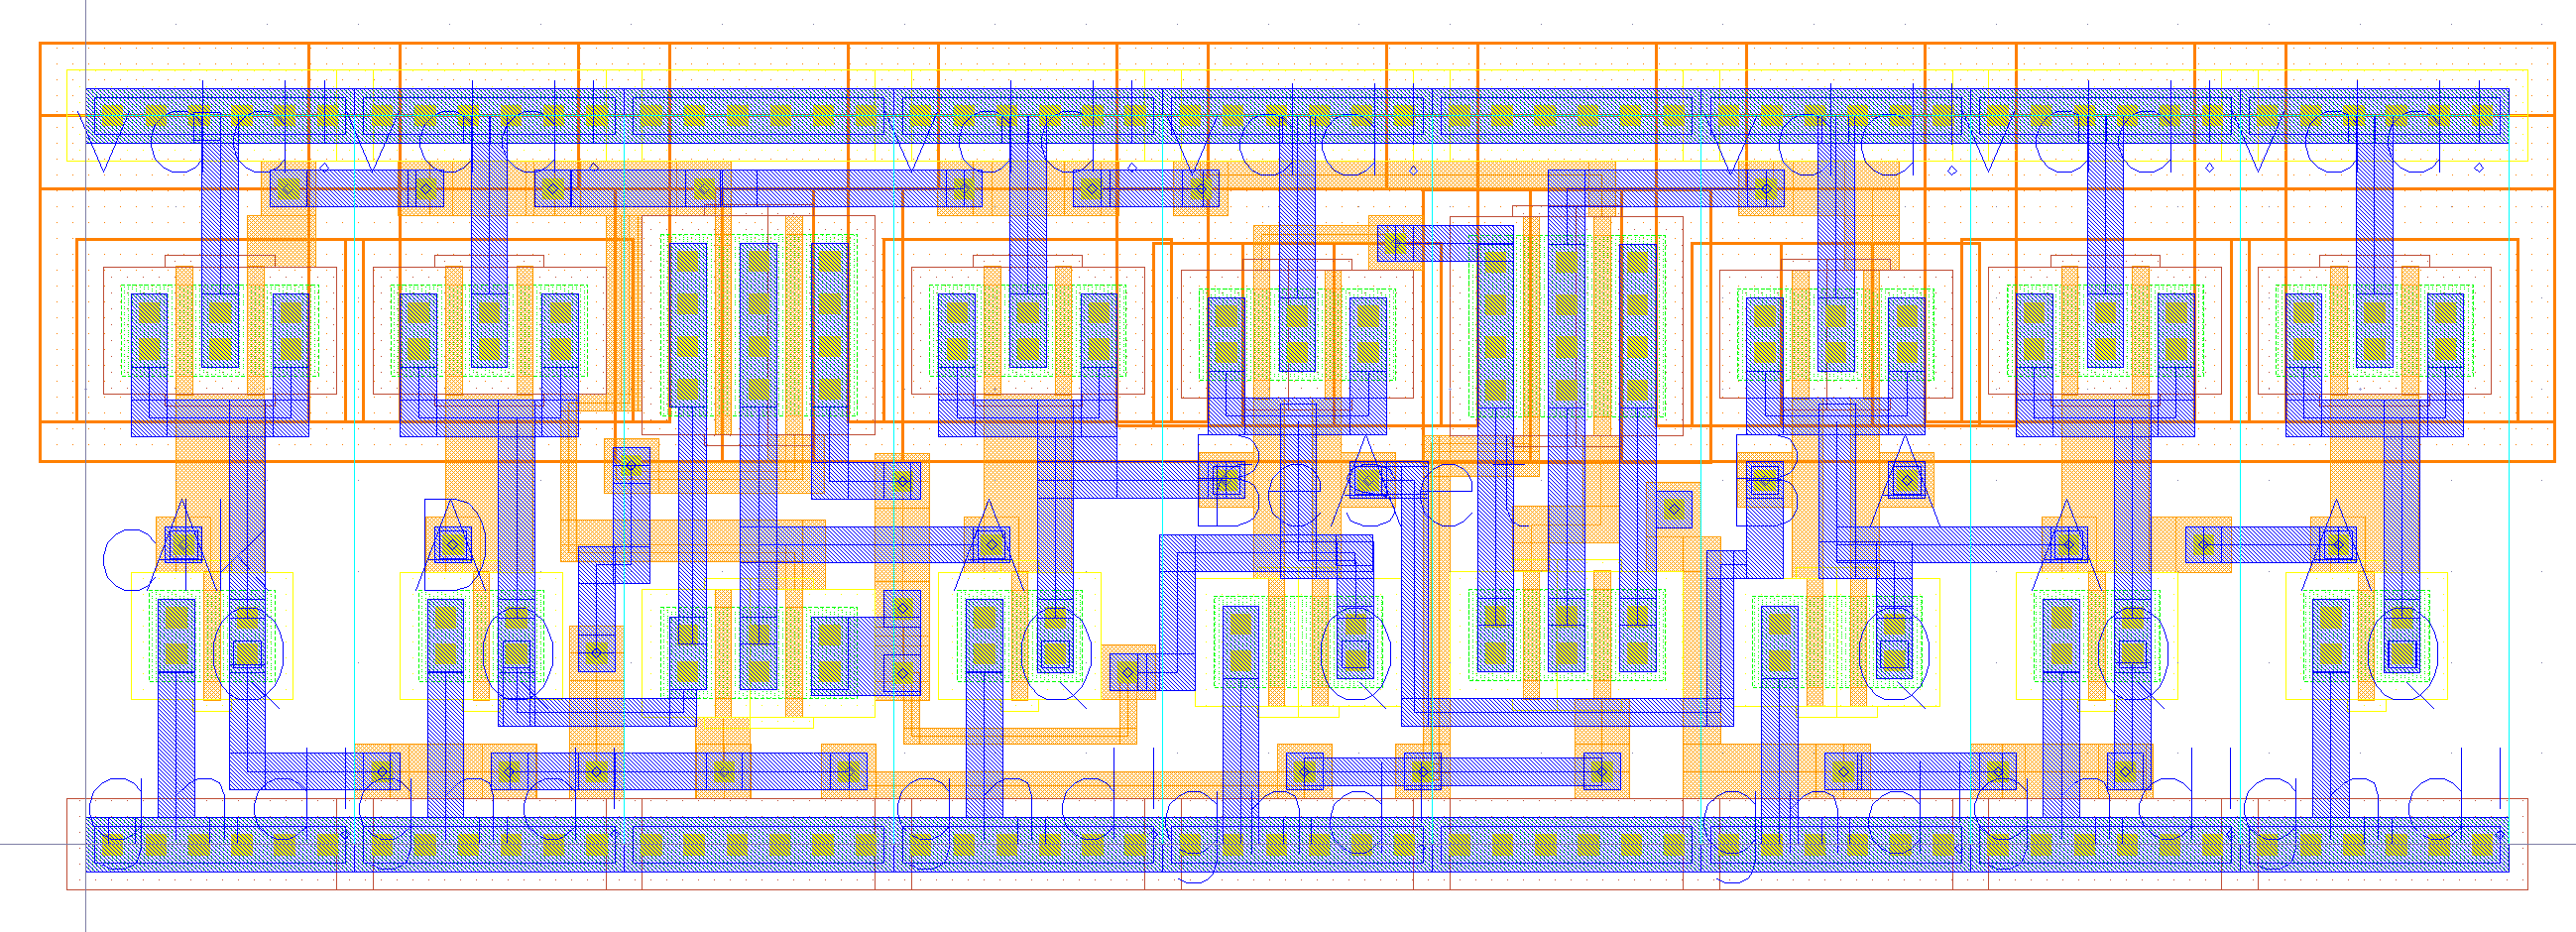
\includegraphics[width=\textwidth]{DFF_lay}
	\caption{Final layout design of DFF cell}
	\label{fig:dff_lay}
\end{sidewaysfigure}
